\documentclass{beamer}
%\usepackage[latin1]{inputenc}
%\usepackage{lmodern}
\usepackage{times}
\usepackage[T1]{fontenc}
\usepackage{graphicx}
\usepackage{bm}
\usepackage[small,labelformat=empty]{caption}

%\usetheme{Frankfurt}
\usetheme{Warsaw}
\title[AllColoursAreBeautiful@27c3]{All Colours Are Beautiful\\ interactive lightinstallation inspired by blinkenlights$\mu c^{3}$}
\author{fpletz, lilafisch}
\institute{from $\mu c^{3}$}
\date{2010-12-29 - Day 3, 27C3}
\begin{document}

\begin{frame}
\titlepage
\end{frame}

\begin{frame}
\frametitle{Outline}
\tableofcontents
\end{frame}
\setlength\fboxsep{5pt}
\setlength\fboxrule{0pt}
\section{$\mu c^{3}$ - local ccc group in munich}
  \begin{frame}{$\mu c^{3}$}
    \begin{columns}%[t]
      \begin{column}{5cm}
        \begin{block}{info}
         Chaos Computer Club M\"unchen
	       \begin{itemize}
            \item e.V. founded in 1999
       	    \item > 80 members
	          \item http://muc.ccc.de
	          \item info@muc.ccc.de
    	    \end{itemize}
        \end{block}
%         \begin{figure}
%          \begin{center}
%          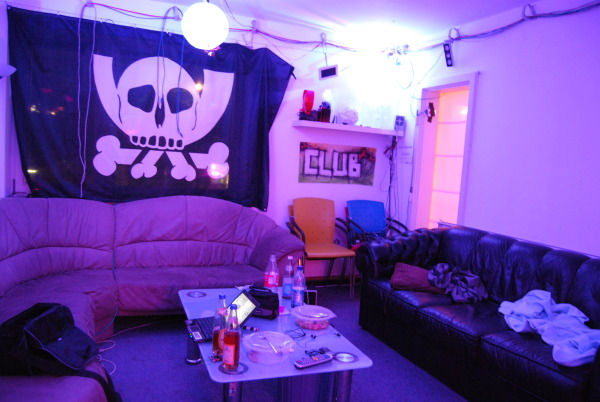
\includegraphics[width=5cm]{bilder/hbf.jpg}
%          \end{center}
%        \end{figure}
 
%         \begin{figure}
 %           \begin{center}
 %           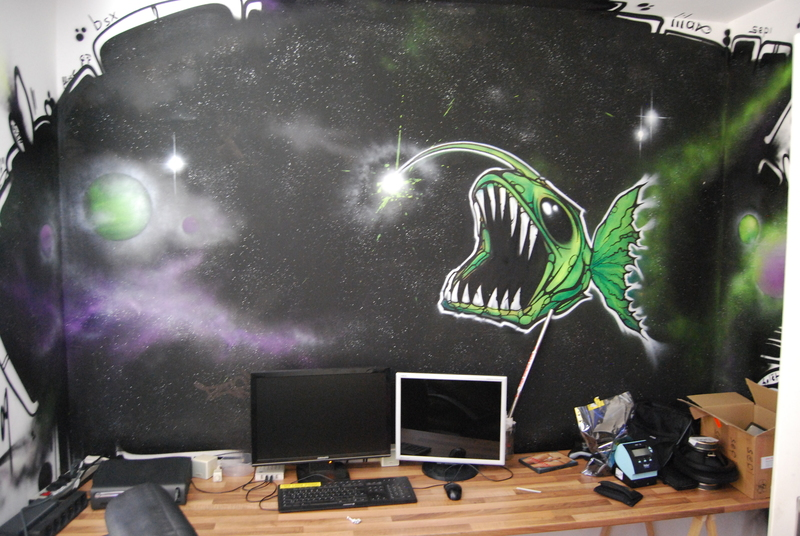
\includegraphics[width=2cm]{bilder/maxi.jpg}
 %           \end{center}
 %         \end{figure}
      \end{column}
      \begin{column}{5cm}
        \begin{figure}
          \begin{center}
          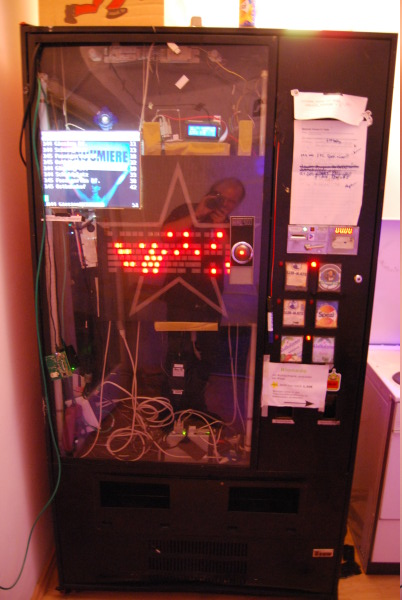
\includegraphics[width=4cm]{bilder/matemat.jpg}
%         \caption{\small matemat}
          \end{center}
        \end{figure}
%        \begin{figure}
%          \begin{center}
%          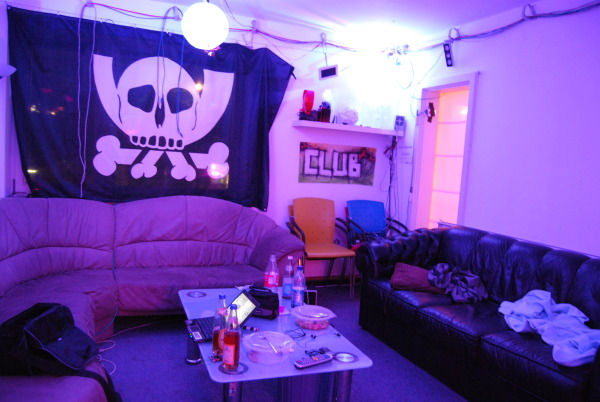
\includegraphics[width=3cm]{bilder/hbf.jpg}
%          \end{center}
%        \end{figure}
      \end{column}
    \end{columns}
    \end{frame}
\section{How it came together}
\begin{frame}{How it came together}

\begin{columns}%[T]
\begin{column}{3.5cm}
        \begin{figure}
          \begin{center}
          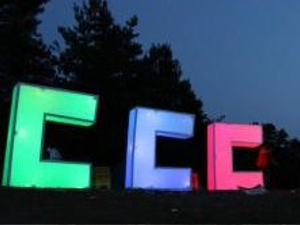
\includegraphics[width=3cm]{bilder/ddc_har.jpg}
          \caption{Moodlamp}
         % members' RGB-LED project, \\were in use for the 3c
          \end{center}
        \end{figure}
\end{column}
\begin{column}{3.5cm}
        \begin{figure}
          \begin{center}
          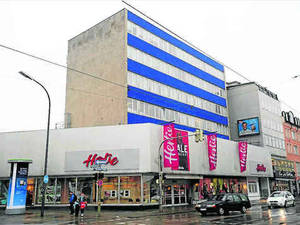
\includegraphics[width=3cm]{bilder/hertie.jpg}
          \caption{Puerto Giesing}
          %old office building,\\used by artists before beeing torn down
          \end{center}
        \end{figure}
\end{column}
\begin{column}{3.5cm}
        \begin{figure}
          \begin{center}
          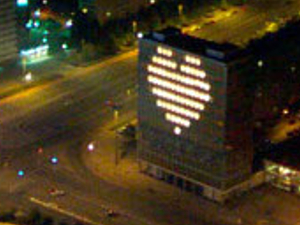
\includegraphics[width=3cm]{bilder/blinkenlights.jpg}
          \caption{Blinkenlights}
          %well known project transforming buildings into b\textbackslash w displays
          \end{center}
        \end{figure}
\end{column}
\end{columns}
\begin{columns}[T]
\begin{column}{3.5cm}
        \begin{figure}
          \begin{center}
          Members' RGB-LED project, \\were in use for the 3c
          \end{center}
        \end{figure}
 
\end{column}
\begin{column}{3.5cm}
        \begin{figure}
          \begin{center}
          Old office building,\\used by artists before beeing torn down
          \end{center}
        \end{figure}
 
\end{column}
\begin{column}{3.5cm}
        \begin{figure}
          \begin{center}
          Well known project transforming buildings into b\textbackslash w displays
          \end{center}
        \end{figure}
 
    \end{column}
\end{columns}
\end{frame}
\section{Hardware}
 \subsection{Development of the Lamp}
  \begin{frame}{a lamp fit for the project}
    \begin{columns}
      \begin{column}{3.5cm}
        \begin{figure}
          \begin{center}
          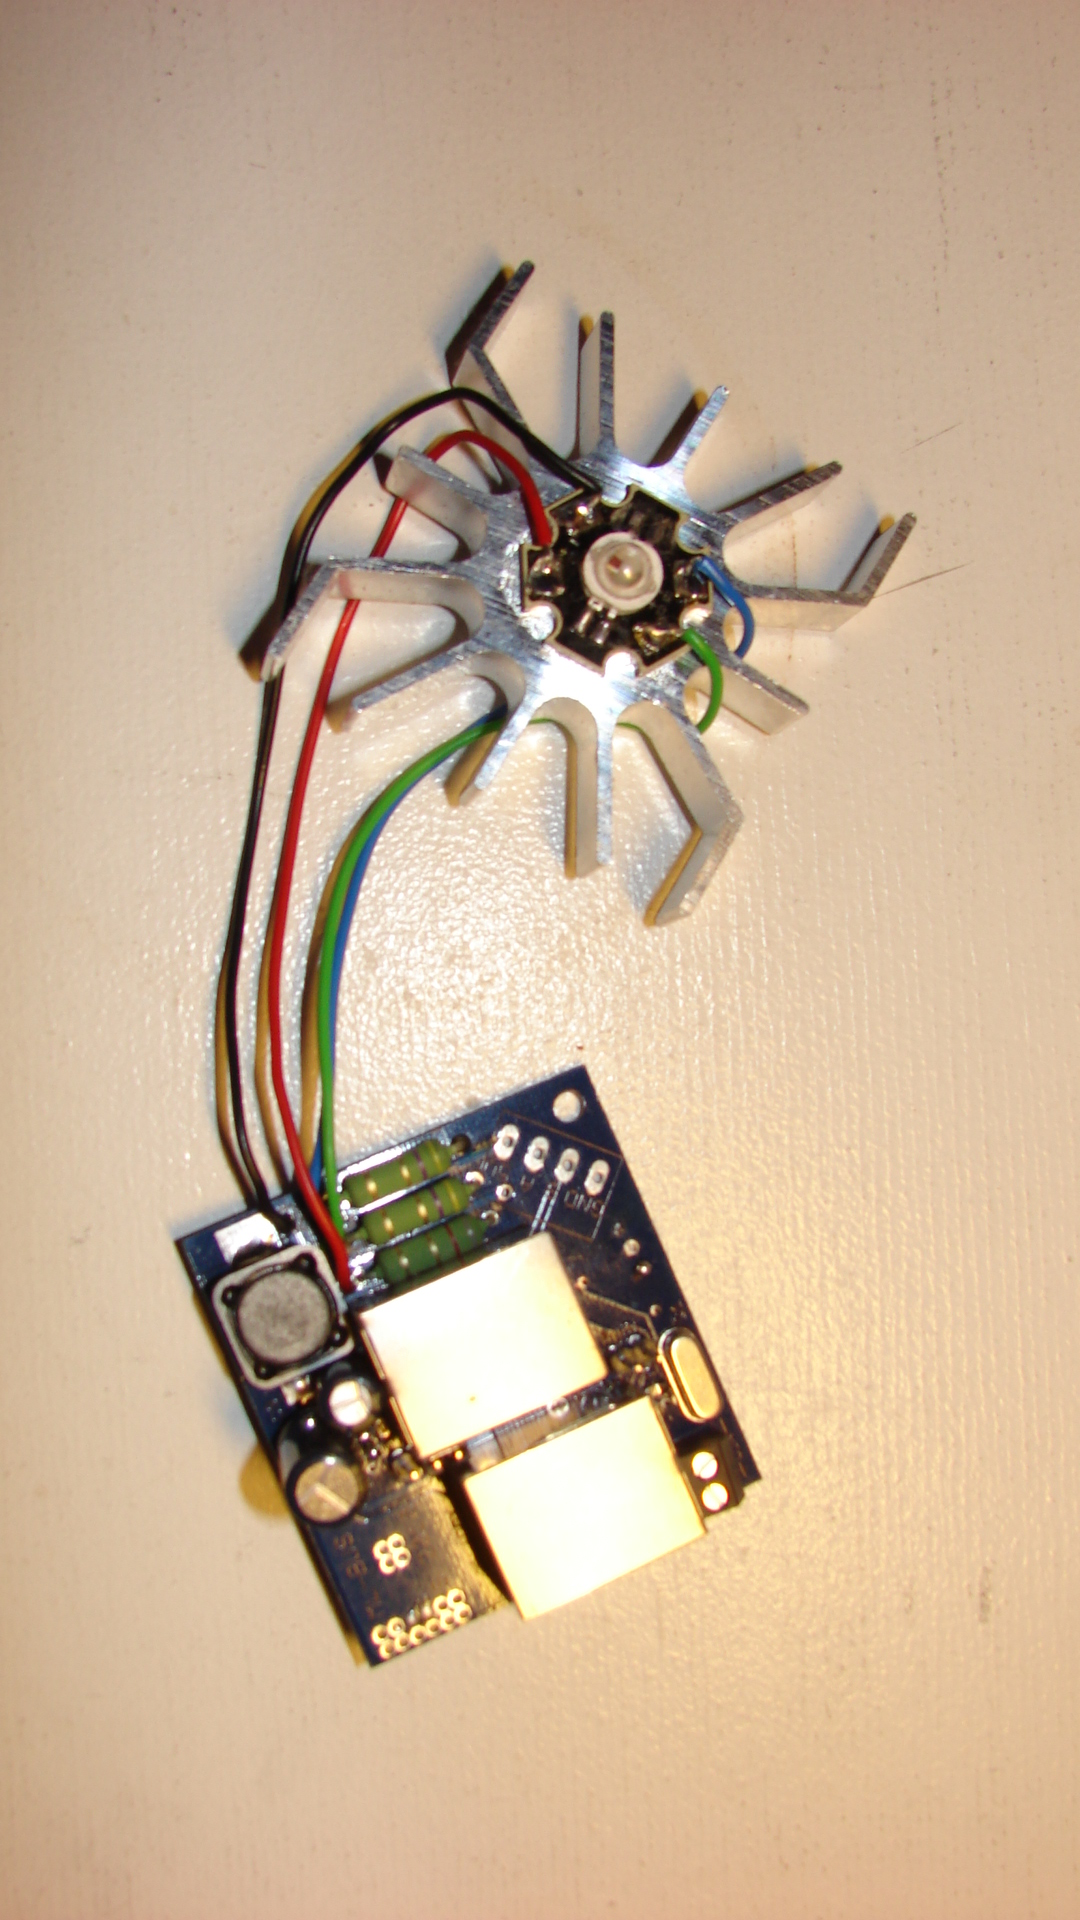
\includegraphics[width=3cm]{bilder/lampe1.JPG}
          \end{center}
        \end{figure}
      \end{column}
      \begin{column}{5cm}
        \begin{itemize}
        \item Not needed ways of communication removed (ir, usb, \ldots)
        \item Switching regulator added for higher supply voltage (-> lower supply current)
        \item Ethernet connectors replace screw terminals for faster and more stable(?) connections 
        \end{itemize}
      \end{column}
      \begin{column}{3.5cm}
         \begin{figure}
          \begin{center}
          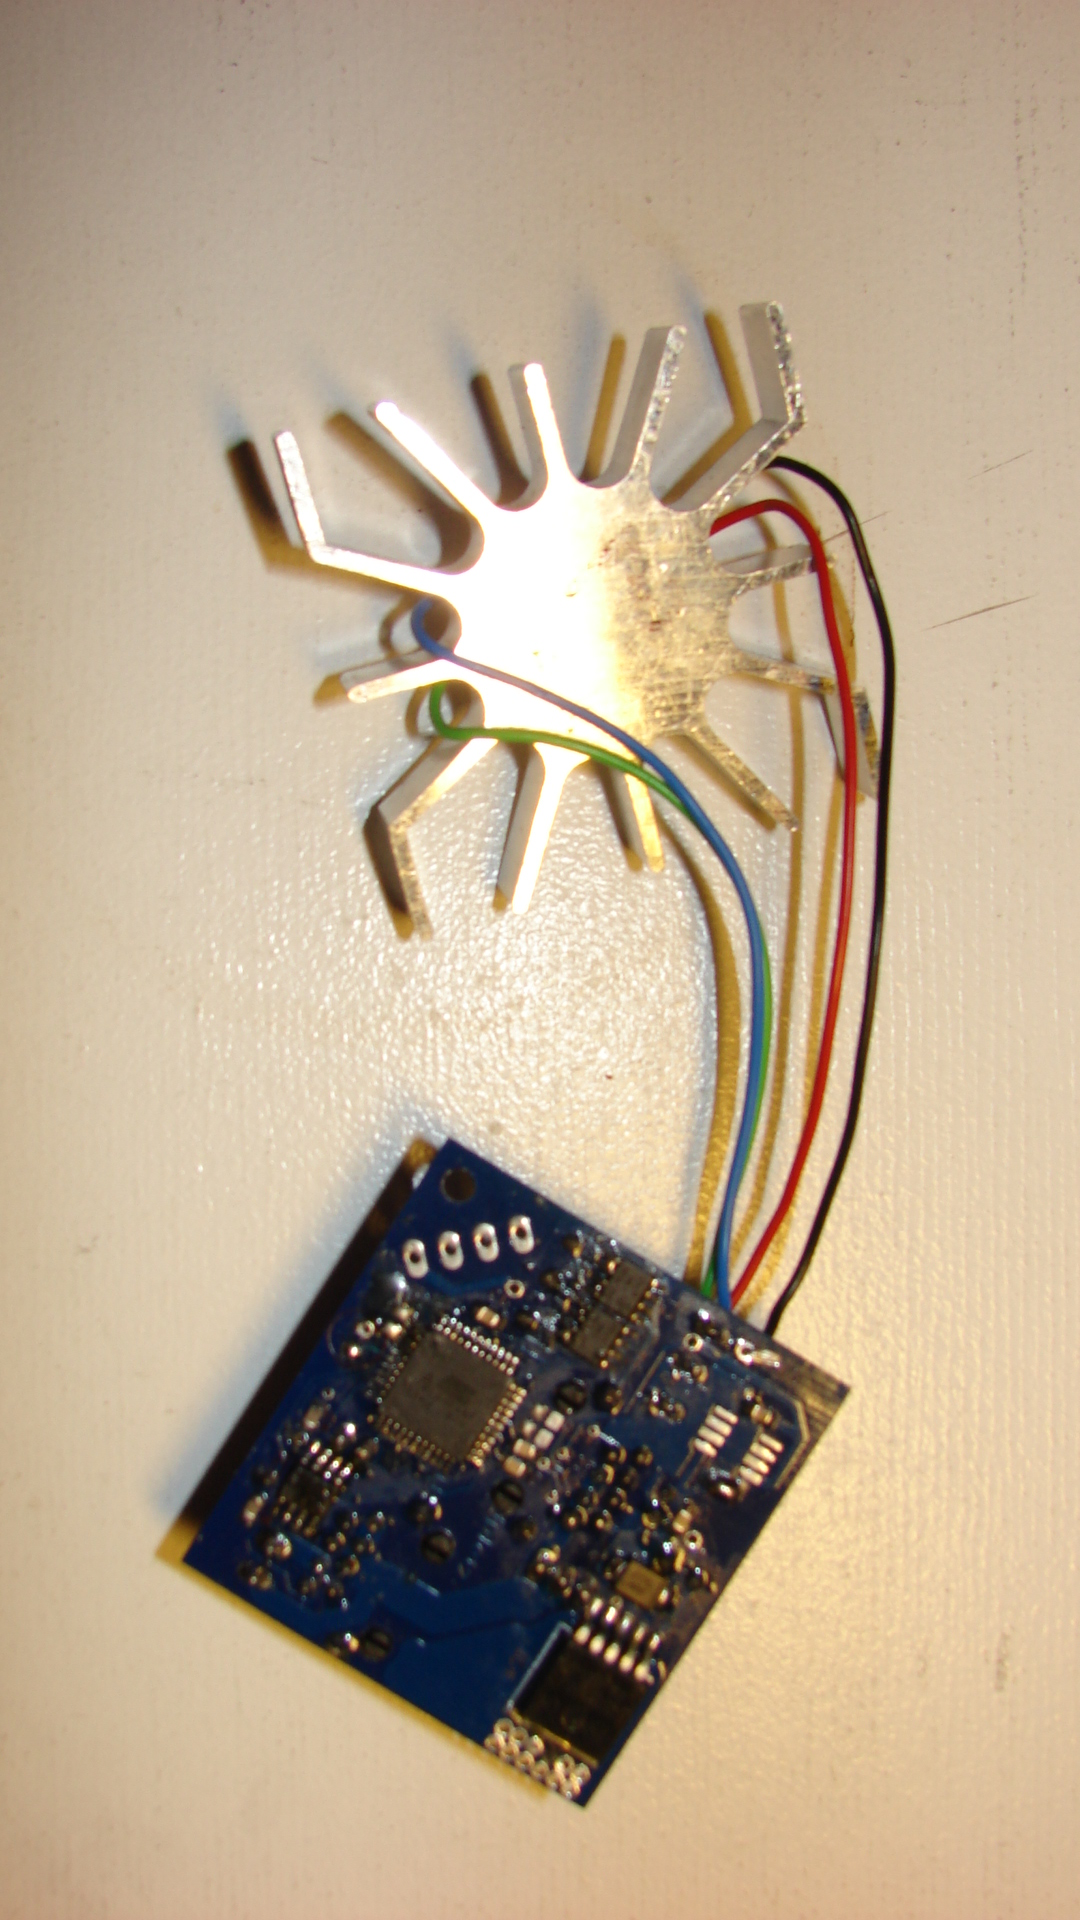
\includegraphics[width=3cm]{bilder/lampe2.JPG}
          \end{center}
        \end{figure}
     \end{column}
    \end{columns}
  \end{frame}
  \begin{frame}{The lamp - Outline}
    \begin{figure}
    \begin{center}
    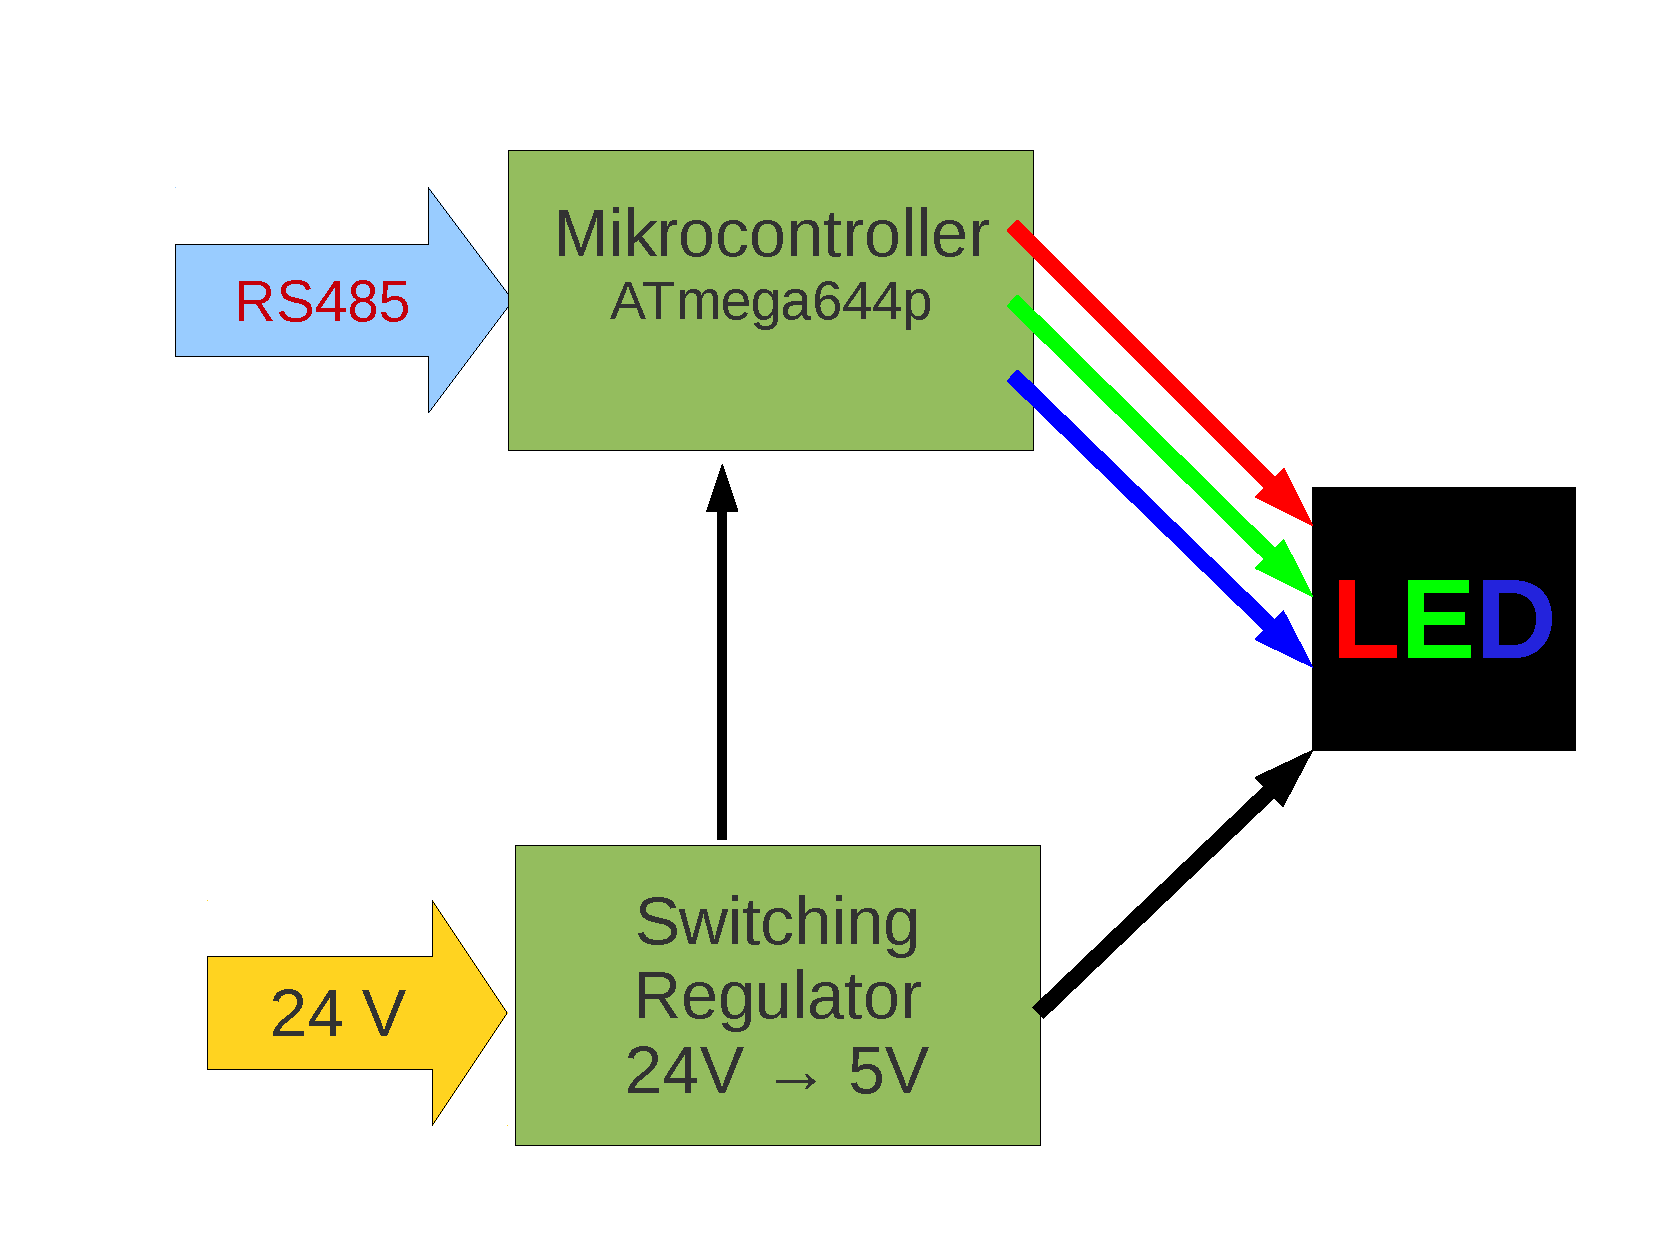
\includegraphics[width=9cm]{bilder/led_12v_rs485.pdf}
    \end{center}
    \end{figure}
  \end{frame}
\subsection{Powersupply}
  \begin{frame}{Powersupply}
  At 12V supplyvoltage the current from one power supply unit suffices for 12 lamps.
  \begin{columns}
    \begin{column}{4cm}
     \begin{block}{ Puerto Giesing}
     Two supply units are used to supply one row
     \end{block}
    \end{column}
    \begin{column}{7cm}
    \begin{figure}
    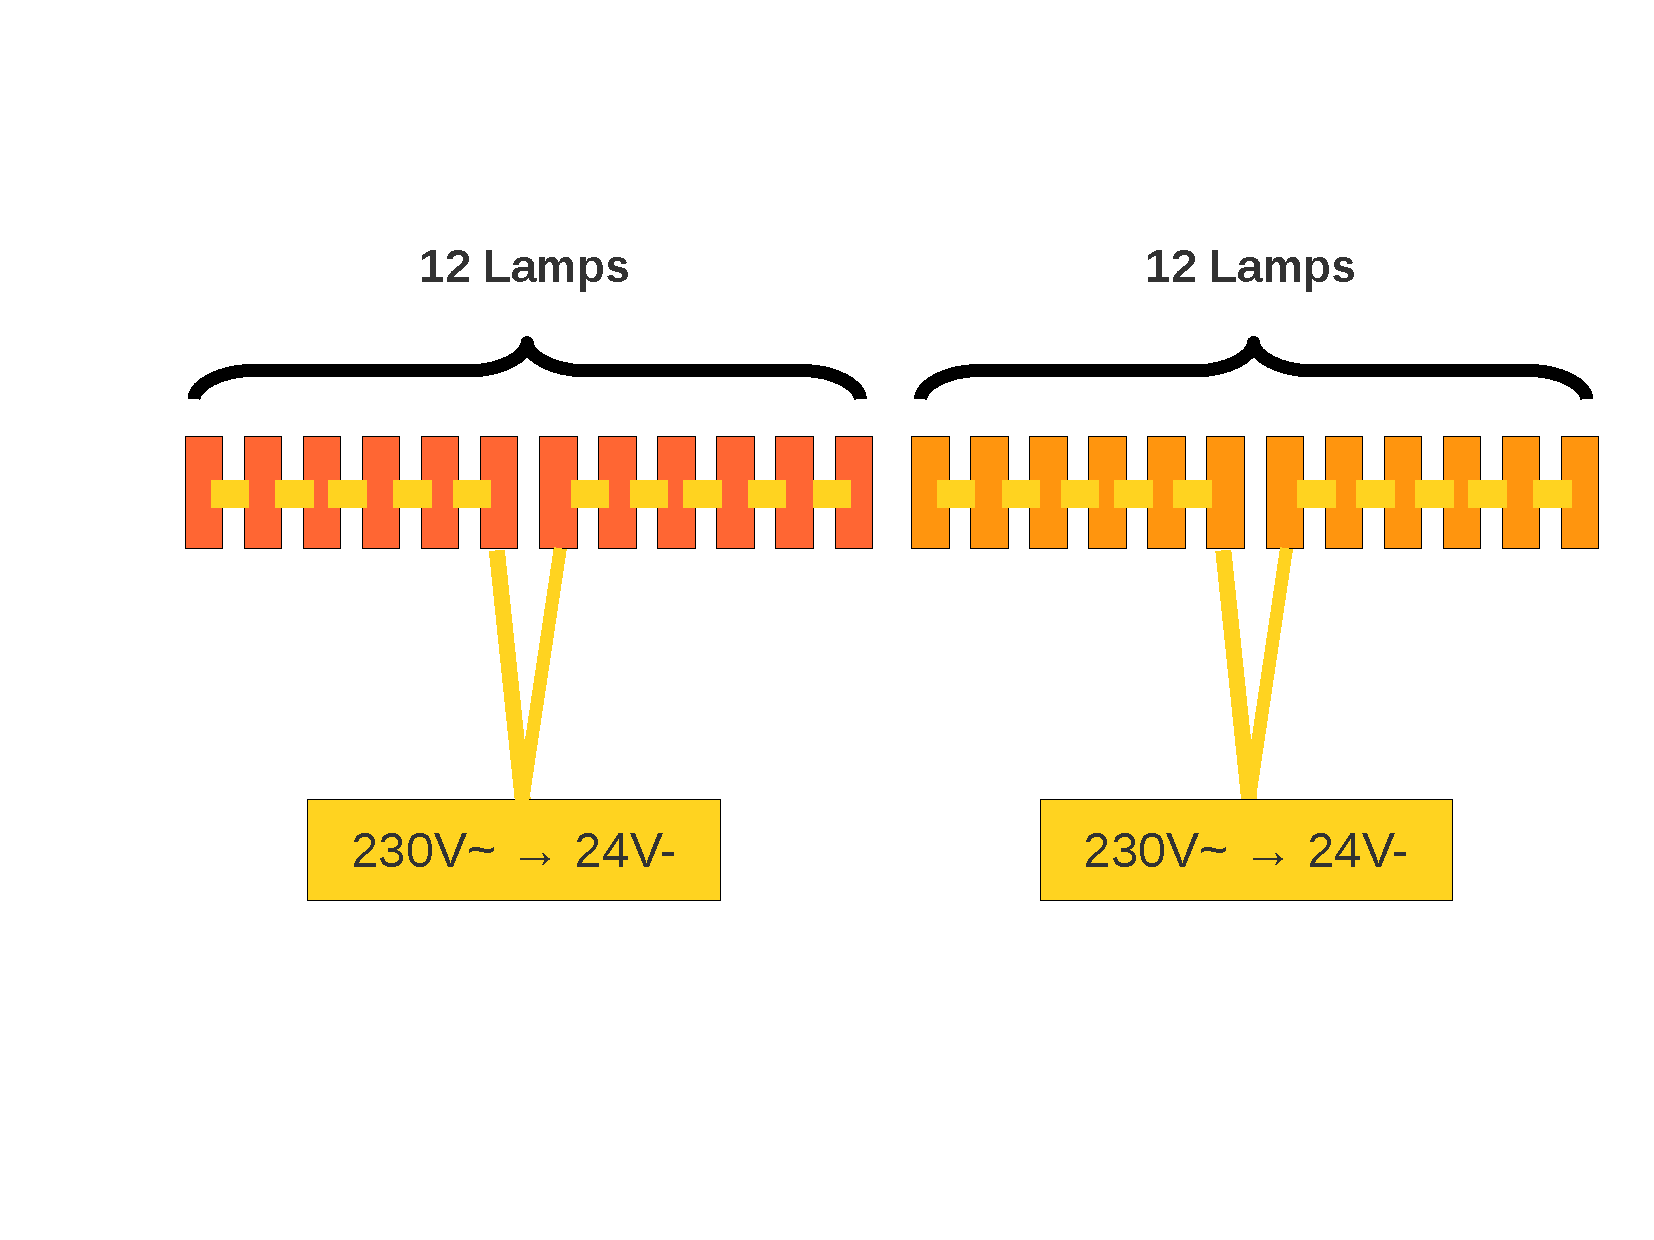
\includegraphics[width=6cm, clip, trim= 2.5cm 4.6cm 0.5cm 4cm]{bilder/12lampen.pdf}
    \end{figure}
    \end{column}
  \end{columns}
  \begin{columns}[T]
    \begin{column}{4cm}
    \vskip 0.4cm 
    \begin{block}{27c3}
     One supply unit is used to supply two columns 
    \end{block}
    \end{column}
    \begin{column}{7cm}
    \begin{figure}
    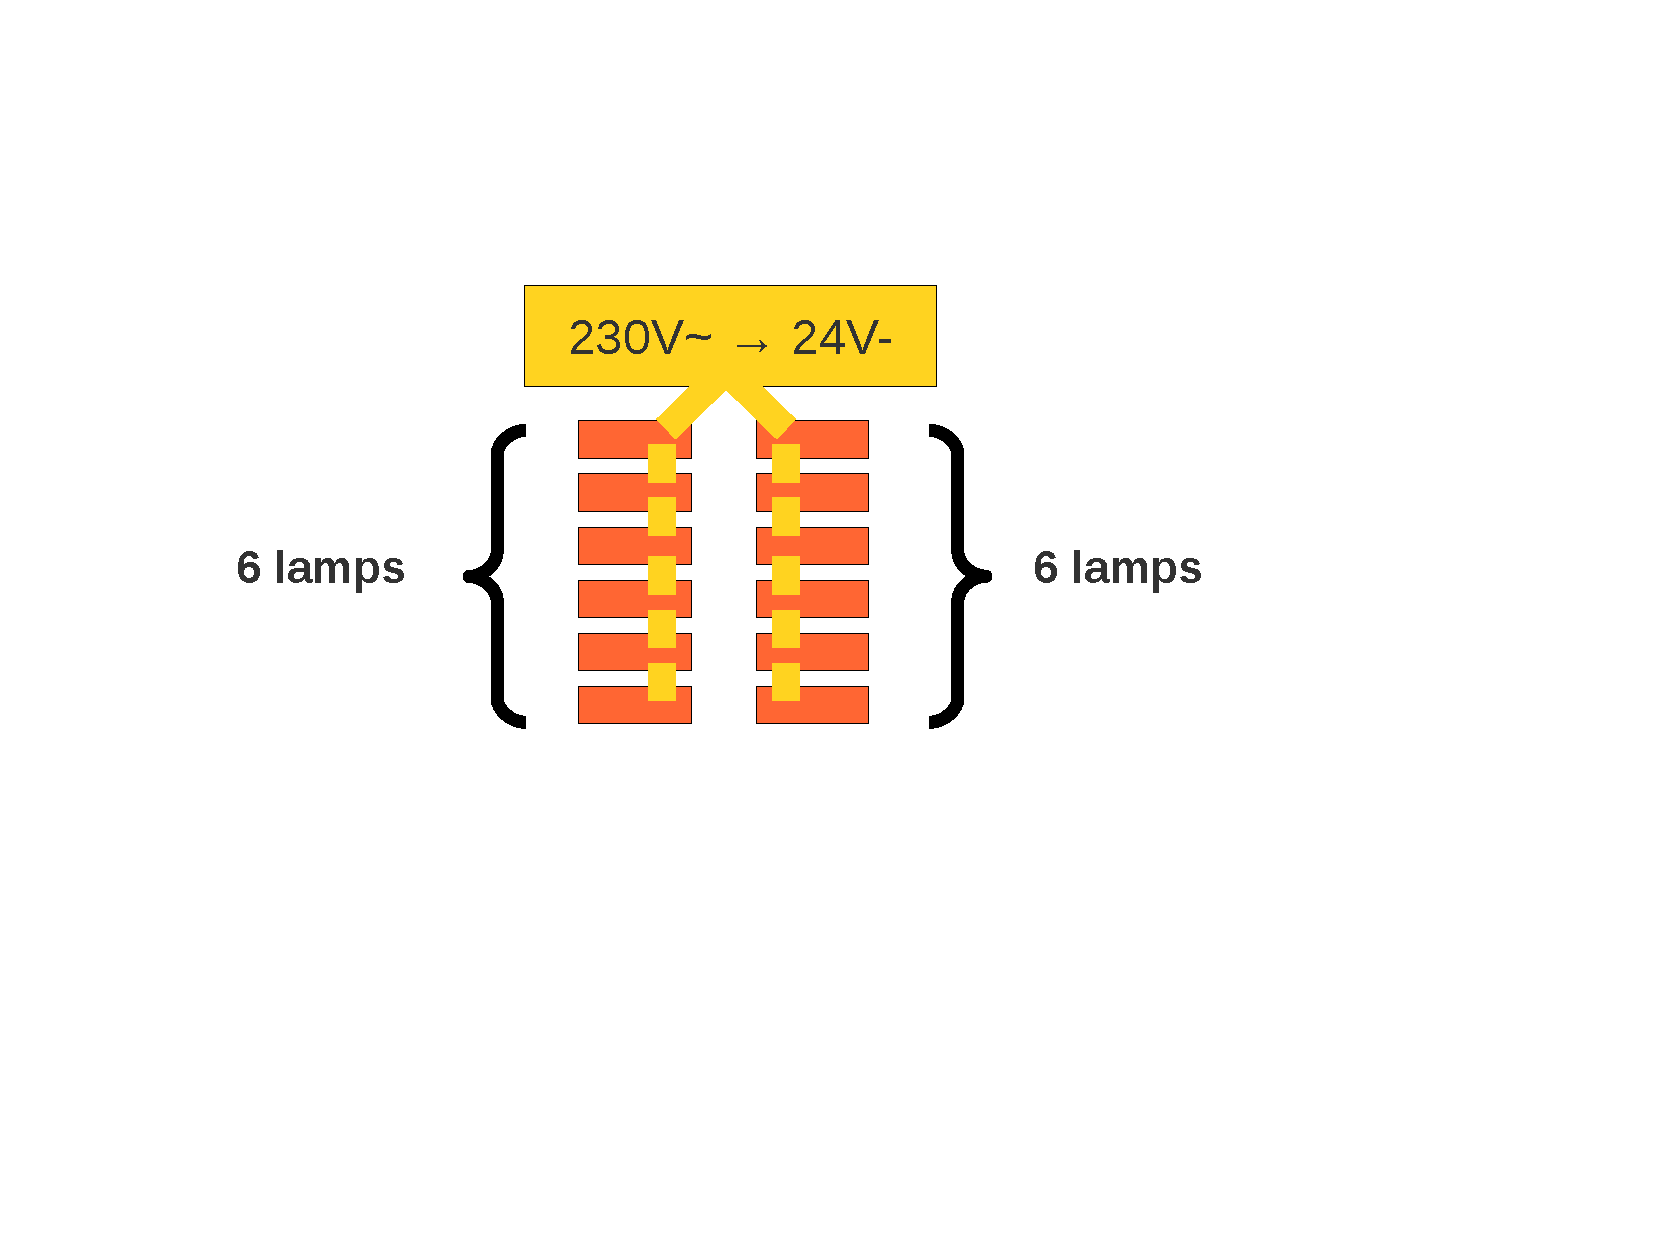
\includegraphics[width=4cm, clip, trim= 4cm 5cm 7cm 4cm]{bilder/6lampen.pdf}
    \end{figure}
    \end{column}
  \end{columns}
  \end{frame} 
\subsection{Dataexchange}
  \begin{frame}{Dataexchange}
    \begin{itemize}
      \item Dataexchange over ethernet cables 
      \item 3 conductor pairs reserved for power supply 
      \item Remaining one used for data
    \end{itemize}
    \begin{columns}[T]
      \begin{column}{7cm}
        \hskip 2.6cm
        Puerto Giesing
        \vskip 0.2cm
        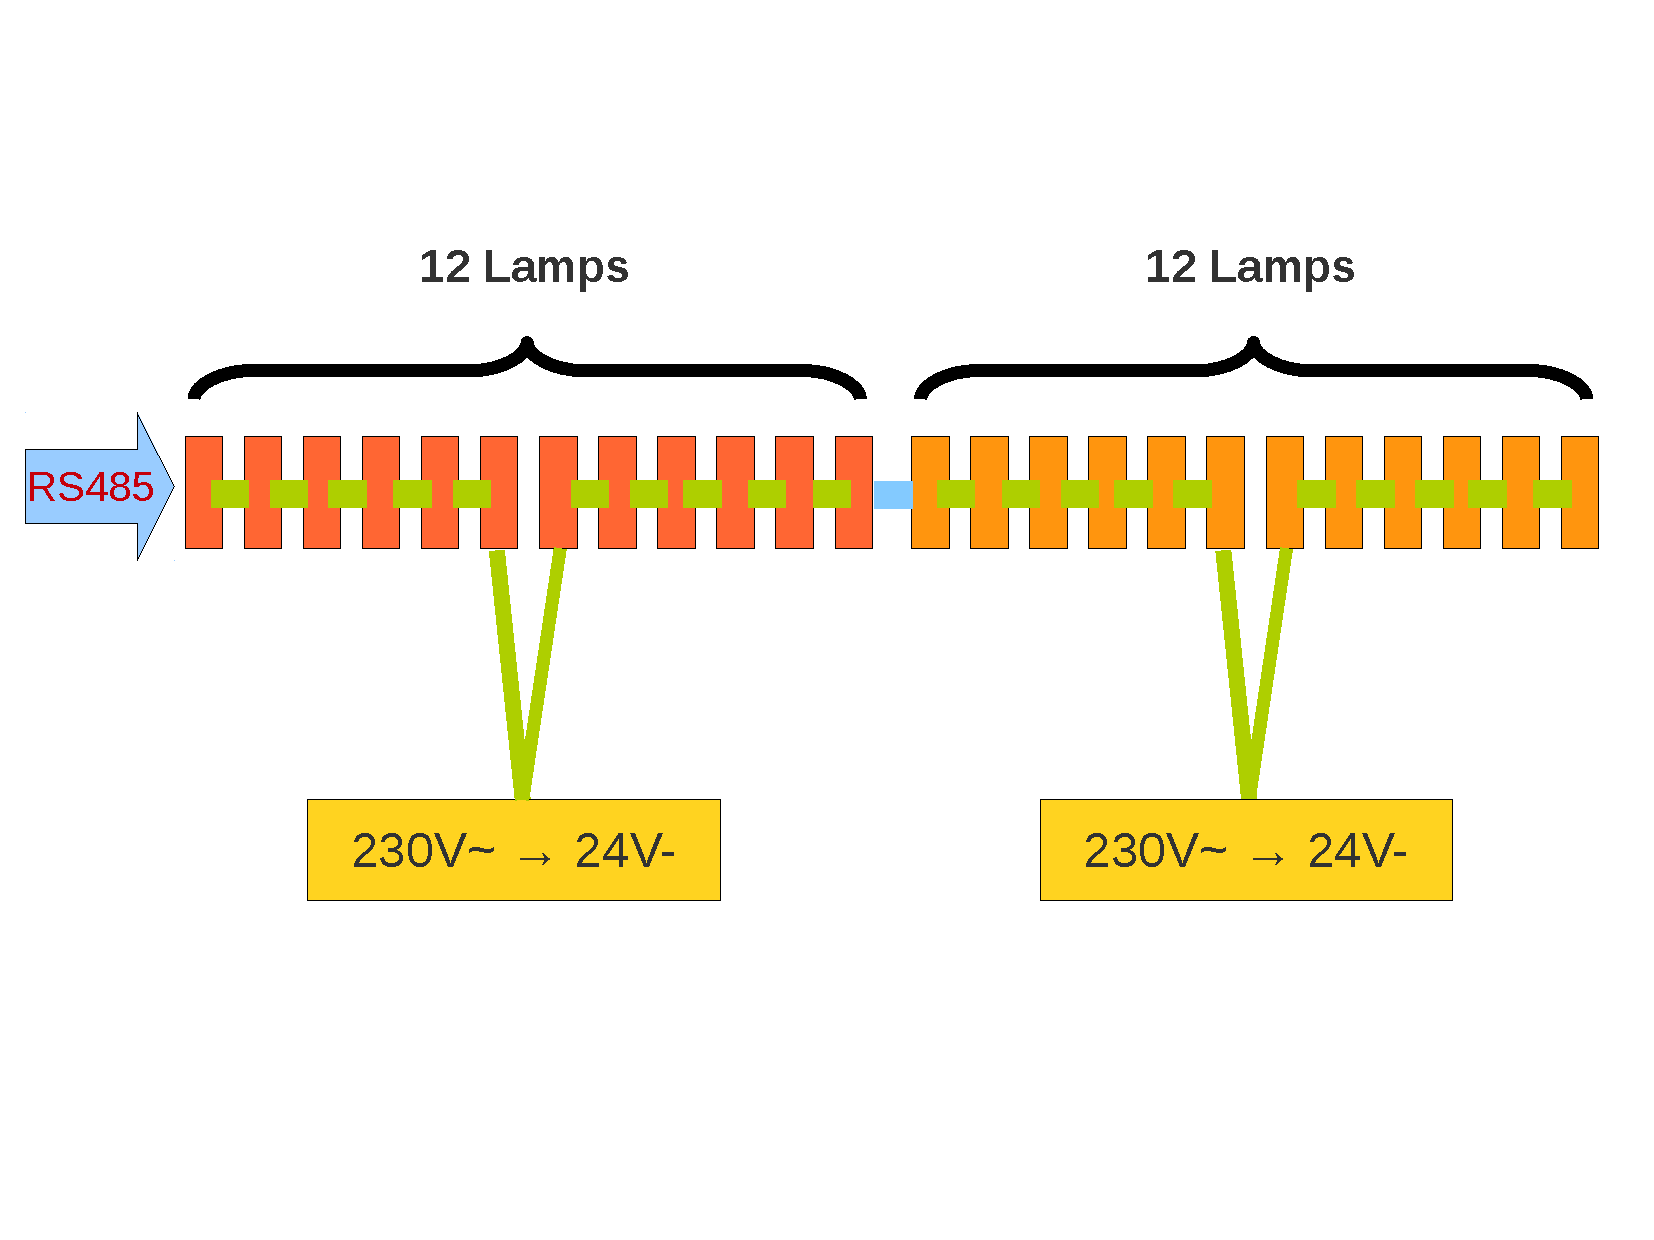
\includegraphics[width=7.3cm, clip, trim= 0cm 4.6cm 0.5cm 4cm]{bilder/12lampen_rs485.pdf}
      \end{column}
      \begin{column}{5cm}
        \hskip 2.0cm
        27c3
        \vskip 0.7cm
         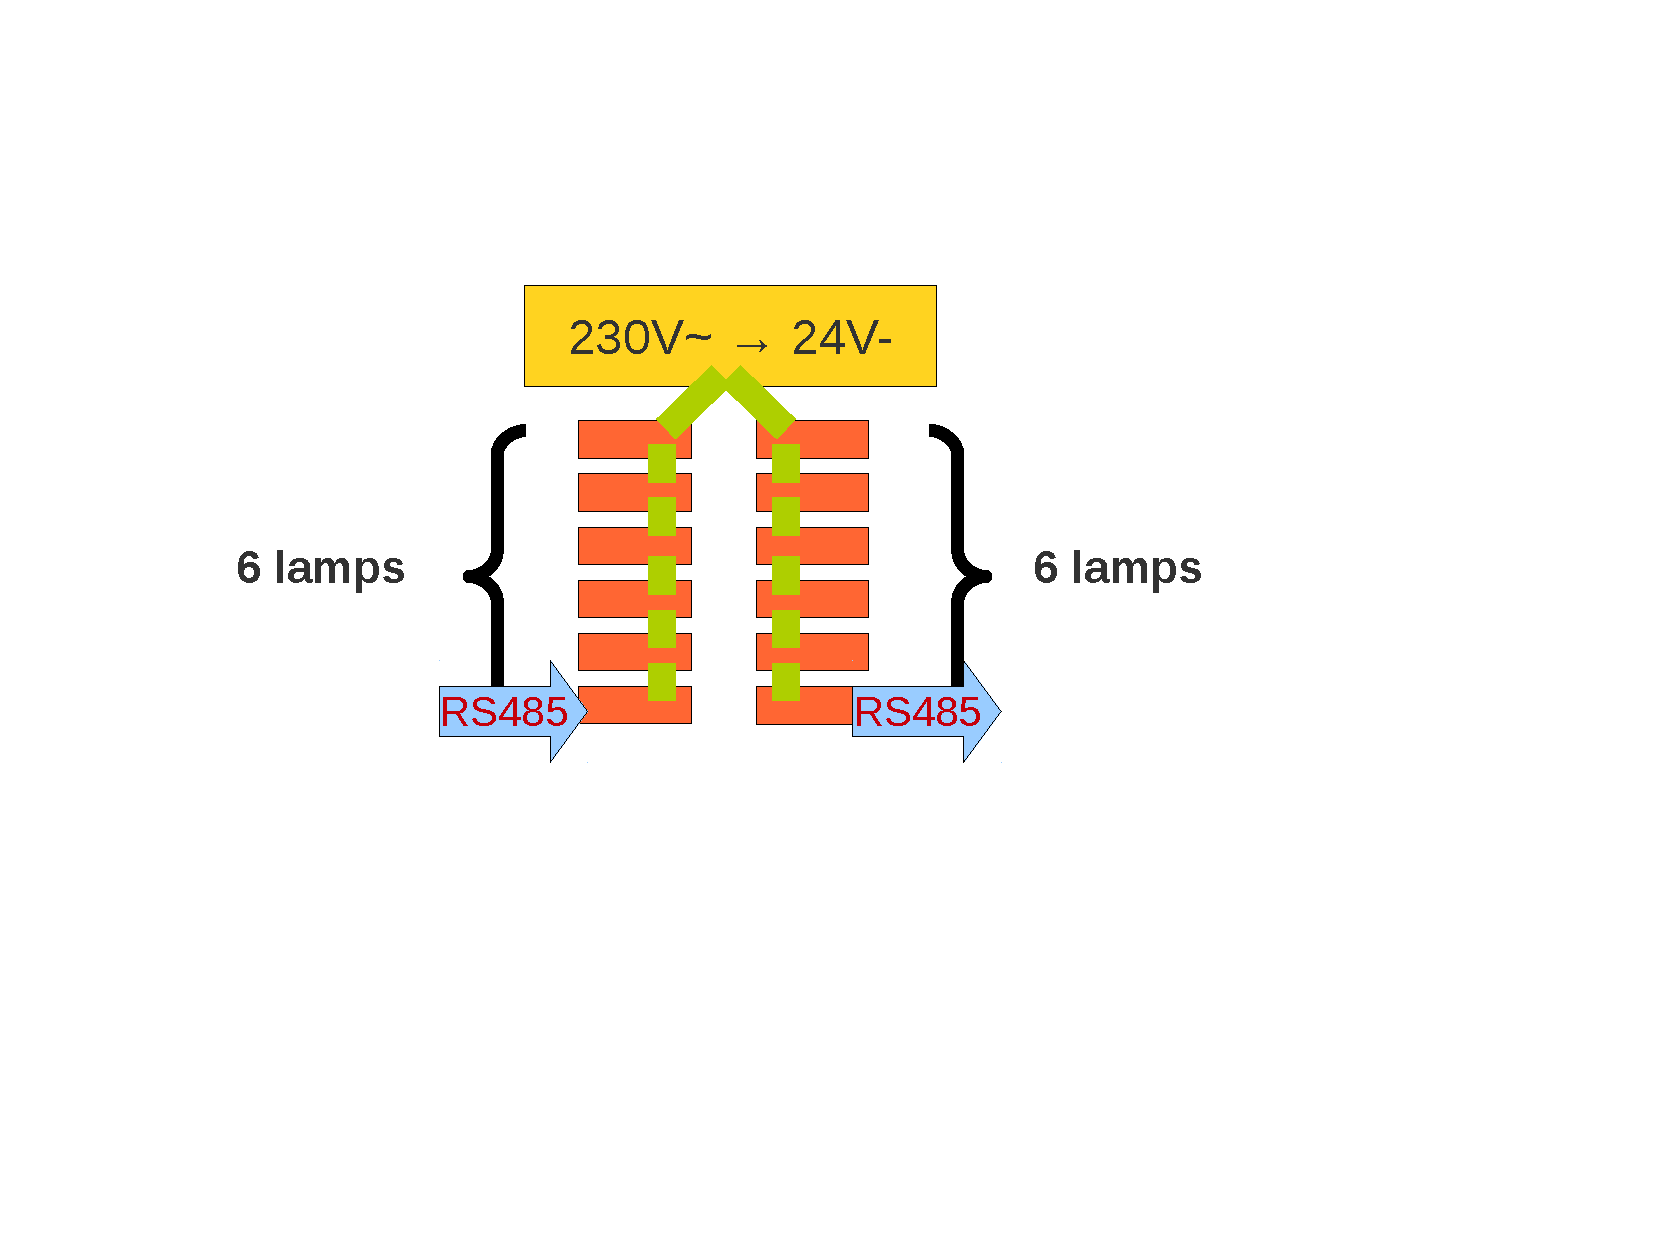
\includegraphics[width=5.5cm, clip, trim= 2.5cm 8cm 3.5cm 4cm]{bilder/6lampen_rs485.pdf}
      \end{column}
    \end{columns}
  \end{frame}
% Was noch fehlt: wie wird das rs485 @congress verteilt
% evtl alles 27c3zeug in section acab@27c3
  \begin{frame}{RS485}
    \begin{columns}
       \begin{column}{6cm}
        \begin{figure}
        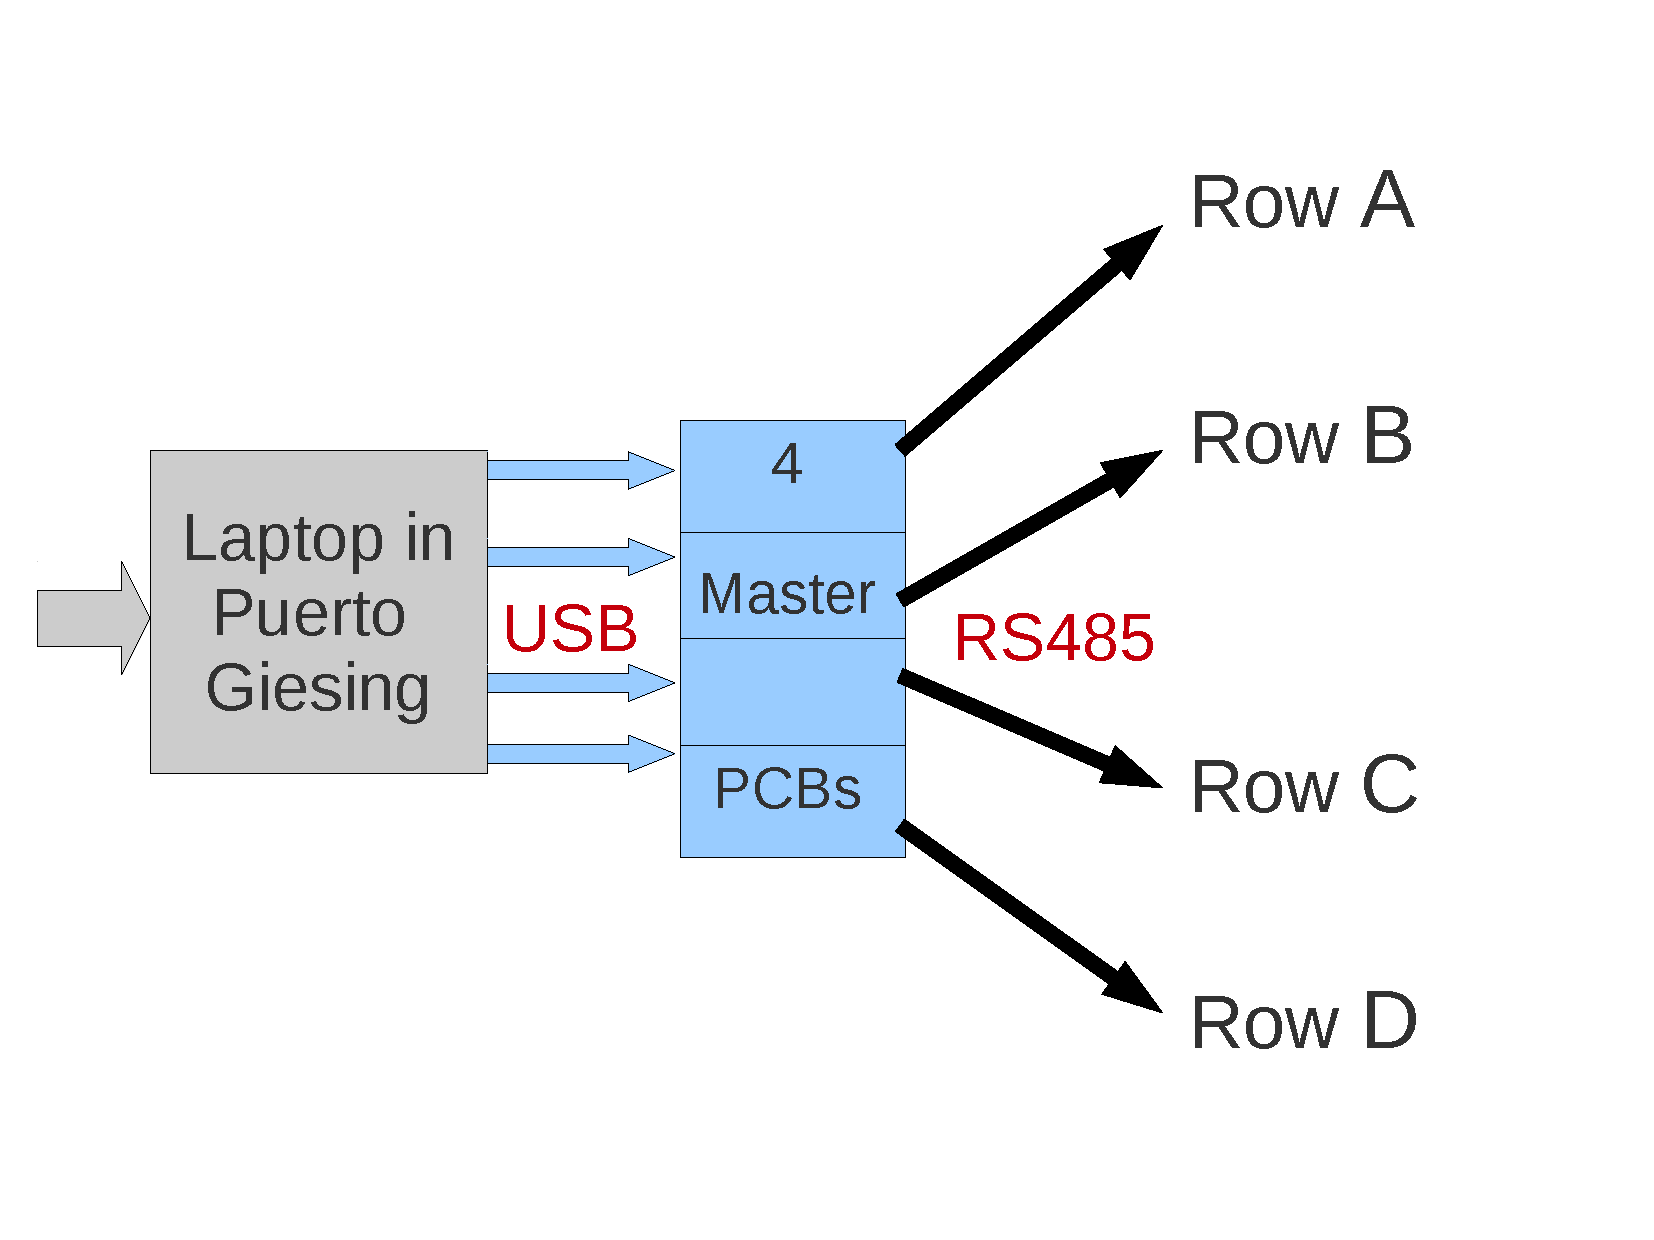
\includegraphics[width=6cm, clip, trim= 1cm 3cm 4cm 2.5cm]{bilder/laptop.pdf}
        \end{figure}
      \end{column}
      \begin{column}{5cm}
      \begin{block}{RS485}
        \begin{itemize}
        \item Versatile communication standard
        \item Vonnects several devices in bus structure
        \item Communication over long distances
        \end{itemize}
      \end{block}
     \end{column}
   \end{columns}
  \end{frame}

\section{Software}
\section{Interaction}
    \subsection{acabed}
    \subsection{Activating Animations by sms}
    \subsection{blubbtris by dasAquarium}
\section{acab@27c3}

\section{acab anywhere}
\section{Contact overview}
\begin{frame}{Contact overview}
  \begin{block}{Information}
    \begin{itemize}
    \item acab.muc.ccc.de
    \item muc.ccc.de
    \item info@muc.ccc.de
    \item presse@muc.ccc.de
    \end{itemize}
  \end{block}
  \begin{block}{Code}
    \begin{itemize}
    \item https://github.com/muccc/acabed
    \item https://github.com/muccc/gigargoyle
    \end{itemize}
  \end{block}
\end{frame}
\end{document}
